\section{Experimentación}

Para las diferentes mediciones necesarias para los experimentos presentados a continuación fueron realizadas sobre una CPU Intel 5200U en un sistema con 8GB de memoria RAM. Los binarios fueron compilados por \texttt{gcc 6.2.1 20160830} utilizando los flags \texttt{-O3 -std=c++11 -march=native}. El toolchain utilizado para correr las mediciones y realizar los gráficos puede encontrarse junto al código en \texttt{tools/data_analisis}.

Para las mediciones de tiempos se corre repetidamente el mismo problema no menos de 4 veces y 100ms para caso, y luego se almacena la media de las mediciones.

\subsection{Runtime de los algoritmos exactos}

\subsubsection{En función de la cantidad de nodos}

En la figura \ref{fig:time-exacto} comparamos el tiempo de ejecución del algoritmo exacto de fuerza bruta con el de backtracking.
Para ello medimos con ambos 5 casos distintos para cada combinación de cantidad de gimnasios y paradas entre 2 y 5. Además usamos siempre un tamaño de mochila mayor a tres veces la cantidad de paradas.

Como podemos observar, los tres se comportan exponencialmente. Sin embargo, es notable la mejora de runtimes tanto al agregar poda de backtracking como al agregar la cota del greedy. Como especulamos en su momento, al contar con una distancia máxima precalculada antes de empezar a hacer backtracking, se logra descartar la suficiente cantidad de ramas como para que justifique el costo del llamado.
\\

Concluímos entonces, a partir de las mediciones, que dicho \emph{tradeoff} está justificado y da buenos resultados.

\begin{figure}[H]
    \centering
    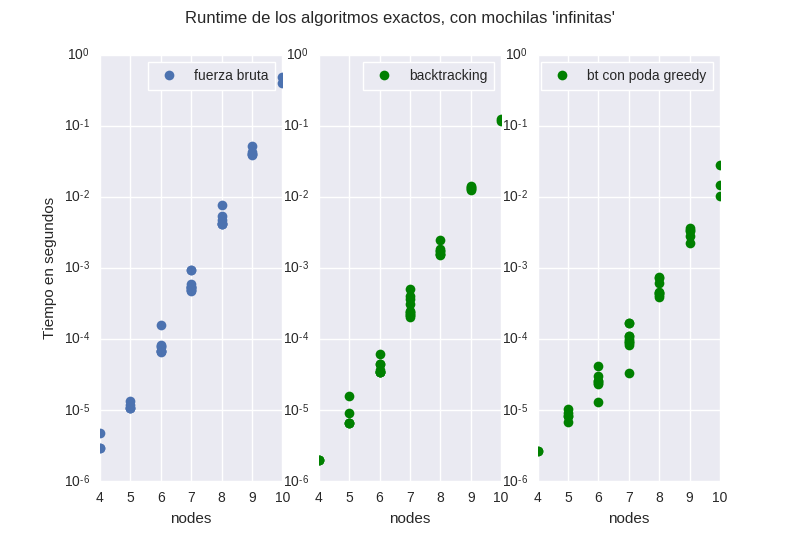
\includegraphics[width=14cm]{time-exacto}
    \caption{Tiempo de ejecución, en escala logarítmica, de los algoritmos exactos.}
    \label{fig:time-exacto}
\end{figure}

\subsubsection{En función del tamaño de la mochila}

A continuación realizamos pruebas fijando la cantidad de gimnasios y paradas en 5 y variando el tamaño de la mochila.

Vemos en la figura \ref{fig:time-exacto-moch} que dentro del intervalo de tamaños de mochila
interesantes, limitado por la cantidad de nodos que puede tener un problema a ser resuelto en un tiempo factible
(ya que si el tamaño es mayor a tres veces la cantidad de paradas, no influirá en el comportamiento del algoritmo) existe una notable diferencia de rendimiento contra la implementación de fuerza bruta a favor de las que usan backtracking.

\begin{figure}[H]
    \centering
    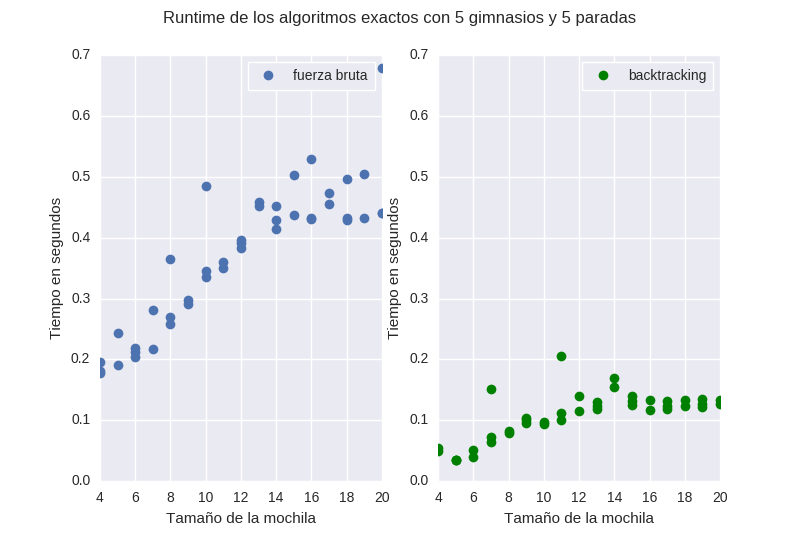
\includegraphics[width=13.5cm]{time-exacto-moch}
    \caption{Tiempo de ejecución de los algoritmos exactos al variar el tamaño de la mochila}
    \label{fig:time-exacto-moch}
\end{figure}

\subsection{Runtime de las heurísticas greedy}

\subsubsection{En función de la cantidad de nodos}

Medimos el tiempo en la figura \ref{fig:time-greedy} generando 5 casos para cada combinación de entre 1000 y 10000 gimnasios y paradas, avanzando de a 1000, y tamaño de mochila mayor a 30000.

Vemos en la figura \ref{fig:time-greedy-correlation} que estos tiempos tiempos se correlaciona fuertemente con un comportamiento cuadrático en función de la cantidad de nodos.

\begin{figure}[H]
    \centering
    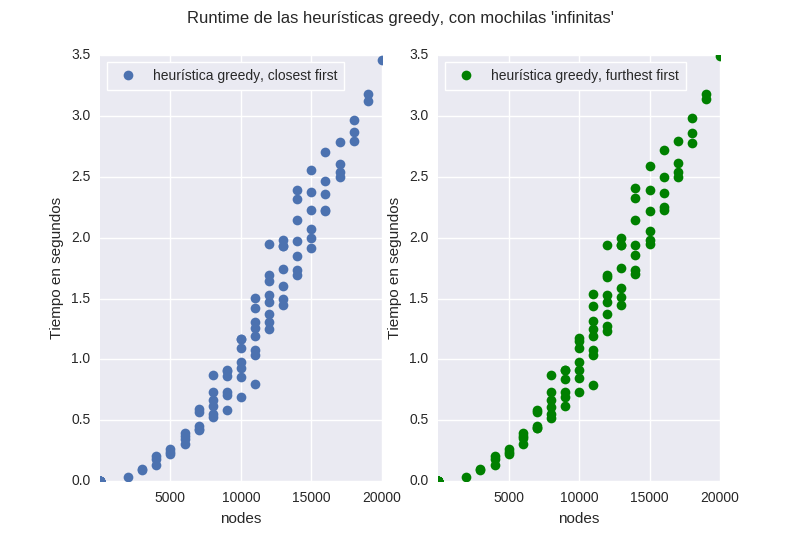
\includegraphics[width=13.5cm]{time-greedy}
    \caption{Tiempo de ejecución de las heurísticas greedy}
    \label{fig:time-greedy}
\end{figure}

Las implementaciones \emph{Closest First} y \emph{Furthest First} mostraron tiempos de ejecuciones notablemente similares, como se aprecia en la figura \ref{fig:time-greedy}. Esto se debe a que el algoritmo es indentico pero modificando el tipo de comparación para elegir el próximo gimnasio (menor distancia por mayor distancia).

\begin{figure}[H]
    \centering
    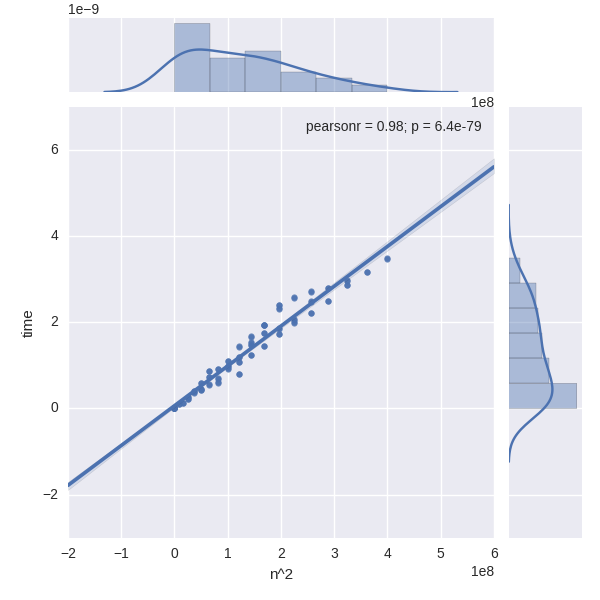
\includegraphics[width=10cm]{time-greedy-correlation}
    \caption{Correlación entre el tiempo de ejecución del greedy y una complejidad cuadrática}
    \label{fig:time-greedy-correlation}
\end{figure}

\subsubsection{En función del tamaño de la mochila}

Realizamos también pruebas fijando la cantidad de gimnasios y paradas en 2500 y variando el tamaño de la mochila entre 100 y 7500 en pasos de a 100, y nos encontramos con un comportamiento constante y con poco ruido para ambos tipos de greedy (con una correlación entre tiempo medido y tamaño de mochila de $0.170856$).

En el cuadro \ref{tab:time-greedy-moch} se encuentra una descripción de los datos medidos.

\begin{table}[H]
    \begin{center}
        \begin{tabular}{ l | r }
            count  & 76.000000 \\
            mean   &  0.215175 \\
            std    &  0.005658 \\
            min    &  0.209863 \\
            25\%   &  0.212328 \\
            50\%   &  0.213131 \\
            75\%   &  0.215283 \\
            max    &  0.239380 \\
        \end{tabular}
        \caption{Descripción de las mediciones en función del tamaño de mochila}\label{tab:time-greedy-moch}
    \end{center}
\end{table}

\subsection{Runtime de las heurísticas locales}

\subsubsection{En función de la cantidad de nodos}

Para las heurísticas locales medimos nuevamente los tiempos generando 5 casos para cada combinación de entre 10 y 100 gimnasios y paradas, avanzando de a 10, y tamaño de mochila mayor a 300. Los resultados se pueden apreciar en la figura \ref{fig:time-local}. Se pasa $corridas=0$, por lo que se itera hasta encontrar un mínimo local.

Podemos corroborar en la figura \ref{fig:time-local-correlation} que ambas variaciones se corresponden con un comportamiento de orden cuarto en función de la cantidad de nodos.

Esto significaría que se hizo una cantidad lineal (también en función de la cantidad de nodos) de llamados a cada método de optimización dado que estos eran cúbicos en complejidad. Magnitud muy distinta a la cota factorial que supusimos en dicha sección, aún cuando considerábamos que era realmente muy poco probable que se tuviera un orden factorial de llamados antes de encontrar un mínimo local.

\begin{figure}[H]
    \centering
    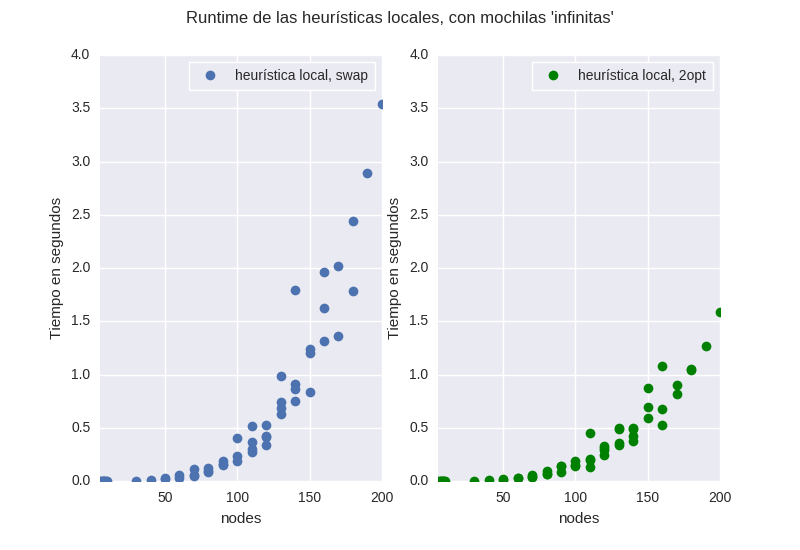
\includegraphics[width=13.5cm]{time-local}
    \caption{Tiempo de ejecución de las heurísticas locales}
    \label{fig:time-local}
\end{figure}

Sobre las instancias más grandes se observa una diferencia favorable hacia $2opt$ respecto de $swap$. Esto lo tendremos en cuenta más adelante a la hora de concluir qué implementación nos dió mejores resultados.

\begin{figure}[H]
    \centering
    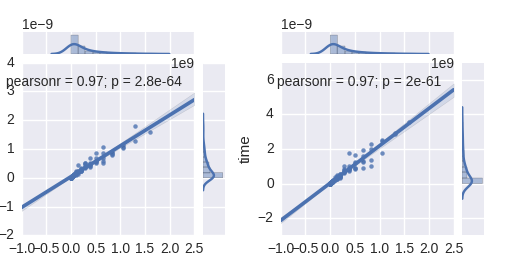
\includegraphics[width=13cm]{time-local-correlation}
    \caption{Correlación entre el tiempo de ejecución de las heurísticas locales 2opt (izquierda) y swap (derecha), con una complejidad $n^4$}
    \label{fig:time-local-correlation}
\end{figure}

    El $swap$ que se tomó para comparar con $2opt$ es aquel que no tomaba el mínimo del vecindario de cada instancia sino que tomaba el primero que tuviera menor distancia a la actual (realizando el resto de las iteraciones sobre el último mínimo encontrado).
    Como especulamos en su momento, al recorrer potencialmente más de un vecindario por iteración (aunque no de manera completa), su performance terminó siendo temporalmente mejor. Esto se ve en la figura \ref{fig:time-local-swap_min} donde se observa un comportamiento de complejidad $n^5$, peor al $n^4$ apreciado en la figura \ref{fig:time-local} correspondiente al $swap$ que se queda con el primer vecino que mejore la distancia.

\begin{figure}[H]
    \centering
    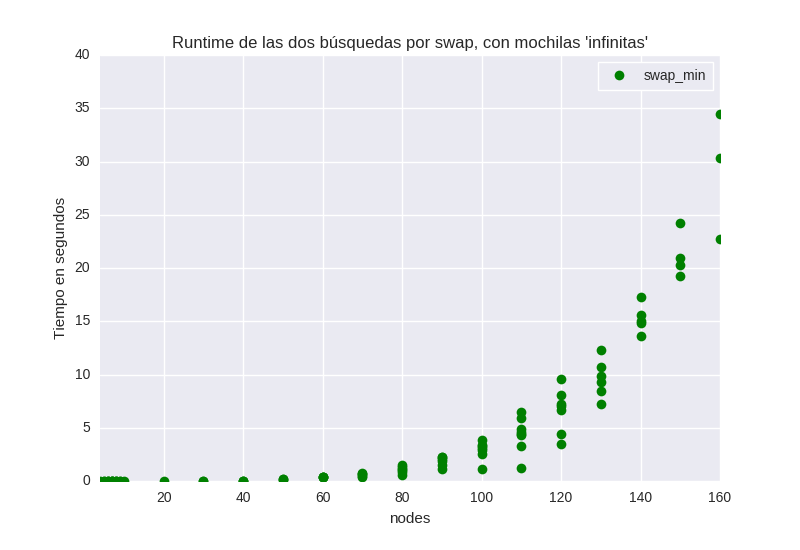
\includegraphics[width=11cm]{swap-min-time}
    \caption{Tiempo de ejecución de la heurística swap tomando el mínimo de cada vecindario por iteración.}
    \label{fig:time-local-swap_min}
\end{figure}

\begin{figure}[H]
    \centering
    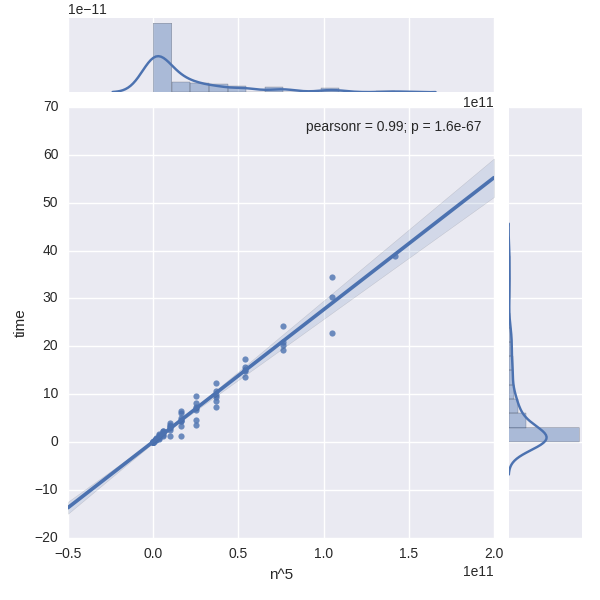
\includegraphics[width=10cm]{swap-min-corr-time}
    \caption{Correlación entre el tiempo de ejecución de la heurística swap tomando el mínimo de cada vecindario por iteración, con una complejidad $n^5$}
    \label{fig:time-local-swap_min-correlation}
\end{figure}

Por lo tanto, utilizamos la otra implementación para el resto de los contrastes empíricos ya que tiene un rendimiento más parecido a la otra búsqueda local implementada, $2opt$, que tampoco tomaba el mínimo de cada vecindario.

\subsubsection{En función del tamaño de la mochila}

Nuevamente realizamos pruebas fijando la cantidad de gimnasios y paradas en 50 y variando el tamaño de la mochila entre 10 y 150, y nos encontramos, al igual que con el greedy, con un comportamiento constante en función de la mochila para ambas variaciones (con una correlación entre tiempo medido y tamaño de mochila de $0.259633$ para swap y de $0.265672$ para 2opt).

En el cuadro \ref{tab:time-local-moch} se encuentra una descripción de los datos medidos.

\begin{table}[H]
    \begin{center}
        \begin{tabular}{ l | r r }
            & Swap & 2opt \\
            \hline
            count  & 141.000000 & 141.000000 \\
            mean   &   0.263016 &   0.167931 \\
            std    &   0.080163 &   0.034468 \\
            min    &   0.124284 &   0.087849 \\
            25\%   &   0.214029 &   0.143264 \\
            50\%   &   0.253680 &   0.165566 \\
            75\%   &   0.297979 &   0.193758 \\
            max    &   0.566984 &   0.268200 \\
        \end{tabular}
        \caption{Descripción de las mediciones en función del tamaño de mochila}\label{tab:time-local-moch}
    \end{center}
\end{table}

\subsection{Runtime de la metaheurística GRASP alternando busquedas locales}
Más adelante, en la subsección \emph{'Variación de las variables del GRASP'} veremos que la precisión de las búsquedas locales en el GRASP alcanza un máximo con un valor finito de iteraciones en cada búsqueda, no siendo necesaria la iteración indefinida hasta alcanzar mínimos locales. Por lo tanto, para medir runtimes, decidimos usar de manera estándar la versión de GRASP alternado, que, a diferencia de la implementación basada en 2opt, itera una cantidad máxima de veces indicada como parámetro teniendo siempre mejores runtimes.

\label{sec:time-grasp}

\subsubsection{En función de la cantidad de nodos}

Para medir el comportamiento de GRASP generamos 4 instancias para cada combinación de gimnasios y mochilas entre 10 y 50, avanzando de a 5, con un tamaño de mochila superior a 150. Además, seteamos ambos exponentes del GRASP en $1$.

En la figura \ref{fig:time-grasp} pueden apreciarse los resultados. Como se observa en la figura \ref{fig:time-grasp-correlation}, el comportamiento está fuertemente correlacionado a un orden 5 sobre la cantidad de nodos.

\begin{figure}[H]
    \centering
    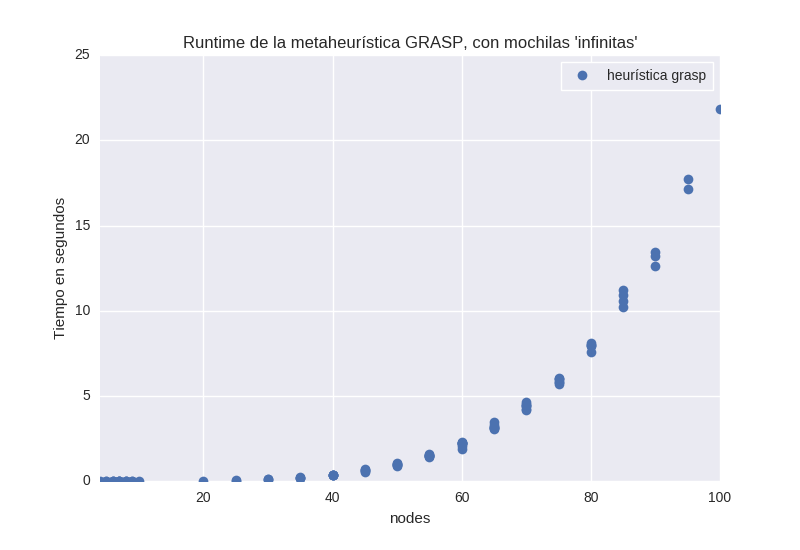
\includegraphics[width=13.5cm]{time-grasp}
    \caption{Tiempo de ejecución de la metaheurística grasp alternando búsquedas locales}
    \label{fig:time-grasp}
\end{figure}

\begin{figure}[H]
    \centering
    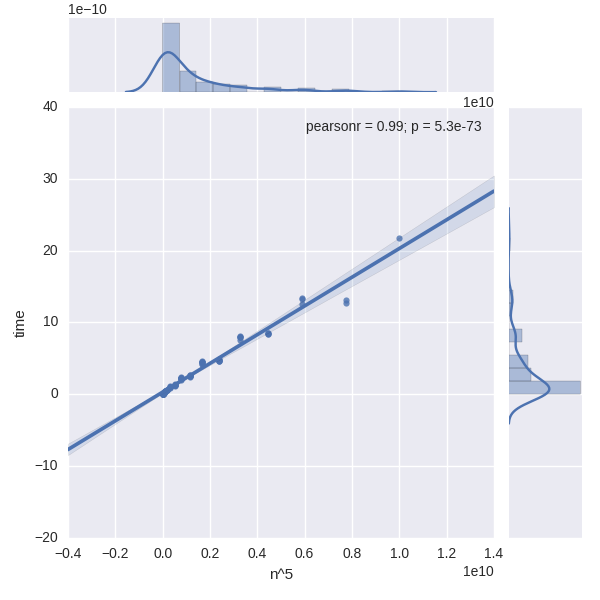
\includegraphics[width=10cm]{time-grasp-correlation}
    \caption{Correlación entre el tiempo de ejecución de grasp alternando búsquedas locales y una complejidad de orden 5 en función de la cantidad de nodos}
    \label{fig:time-grasp-correlation}
\end{figure}

\subsubsection{En función del tamaño de la mochila}

Para medir el tiempo de ejecución en función del tamaño de la mochila fijamos la cantidad de gimnasios y paradas en 20 y variamos la mochila entre 10 y 60. Como se aprecia en la figura \ref{fig:time-grasp-moch}, nos encontramos con que para tamaños pequeños se observa una correlación entre la mochila y el tiempo de ejecución, pero mas o menos a partir del tamaño 30 los tiempos se mantienen relativamente constantes.

Esto puede deberse a que cuando hay poco espacio el la mochila se limita la cantidad de opciones que puede tomar el algoritmo, lo que hace que termine mas temprano.

\begin{figure}[H]
    \centering
    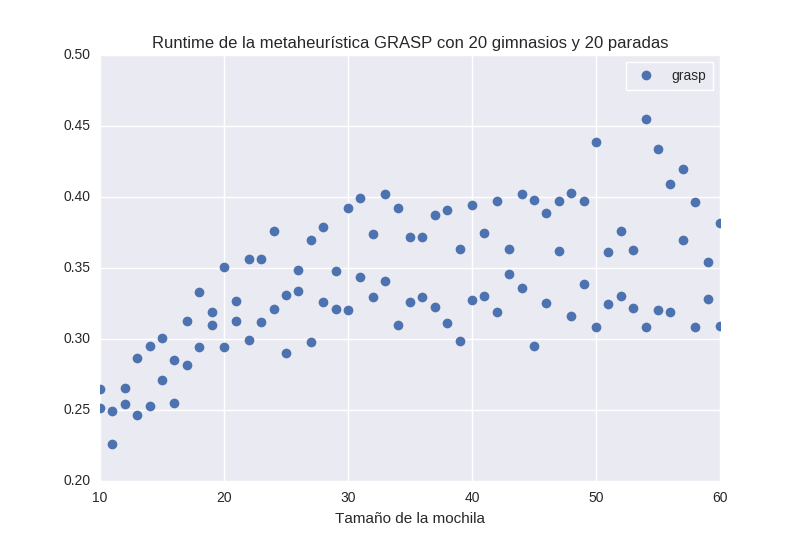
\includegraphics[width=11cm]{time-grasp-moch}
    \caption{Correlación entre el tiempo de ejecución de grasp y una complejidad de orden 5 en función de la cantidad de nodos}
    \label{fig:time-grasp-moch}
\end{figure}

\subsection{Precisión de las heurísticas}

Para medir que tan buenos son los resultados corrimos el mismo problema con cada heurística y comparamos con el resultado real,
obteniendo la proporción entre la solución encontrada y la buscada. Como el nuestro es un problema de minimización,
las proporciones siempre serán mayores o iguales a 1 (nuestras heurísticas siempre encuentran una solución posible).

Para testear problemas de mayor tamaño, tomamos como resultado de comparación el menor valor encontrado entre todas las heurísticas.

\subsubsection{Precisión en casos pequeños, comparando con el exacto}
\label{sec:precision-small}

Para cada combinación de gimnasios y paradas tal que su suma sea menor a 14 (y ambos $\geq 1$) generamos 4 casos usando el generador \texttt{random},
uno con mochila de tamaño 3, otro con tamaño igual a la cantidad de paradas, otro con el doble de las paradas
y uno con espacio igual a trues veces la cantidad de paradas.
Resolvimos estos casos con cada uno de nuestros algoritmos y comparamos las soluciones.

En la figura \ref{fig:precision-small-all} vemos las distribuciones de las precisiones para cada heurística.

Como era de esperar los algoritmos greedy suelen obtener resultados muy por encima del valor óptimo, aunque vemos que en el $75\%$
de los casos la variante closest first obtuvo un valor menor al doble del buscado.
Las heurísticas locales, especialmente la variante swap, mejoraron bastante la precision (a costa de un tiempo de ejecución bastante mas elevado).

Y por último, el GRASP alternado (grasp en la figura) obtuvo el óptimo en un $82.3\%$ de los casos, un poco mejor que la versión 2opt.
En el cuadro \ref{tab:precision-small-grasp} se describe la distribución de su precisión.

\begin{figure}[H]
    \centering
    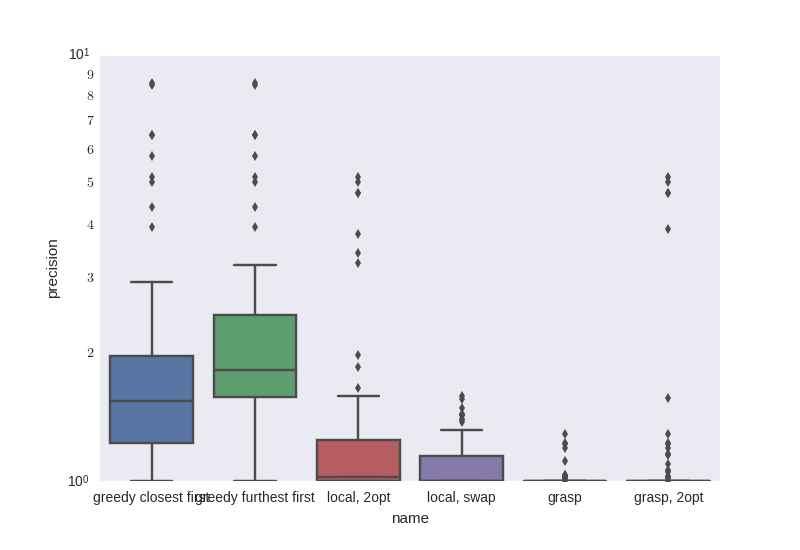
\includegraphics[width=12cm]{precision-small-all}
    \caption{Precisión comparando con el valor mínimo conseguido mediante un algoritmo exacto.}
    \label{fig:precision-small-all}
\end{figure}

Respecto de las heurísticas golosas, comparando a partir la figura \ref{fig:precision-small-all} podemos ver una ventaja, acorde quizás a las expectativas detrás de la intuición de cada heurística, para la implementación \emph{Clostest First} respecto de \emph{Furthest First}.
\\

En el caso de las heurísticas locales,  $2op$ presenta una varianza muchísimo mayor que $swap$ a pesar de que, por debajo de sus terceros cuartiles, las precisión es apenas favorable para esta última.
\\

Para las versiones de GRASP, se ve también una gran varianza en el caso de la basada en $2opt$ (seguramente a causa de la varianza general de dicha búsqueda local, como ya vimos antes). Mientras que las mediciones del GRASP alternado están más concentradas en las cercanías al valor óptimo.

\begin{table}[H]
    \begin{center}
        \begin{tabular}{ l | r }
            count  & 226.000000 \\
            mean   &   1.011650 \\
            std    &   0.039716 \\
            min    &   1.000000 \\
            25\%   &   1.000000 \\
            50\%   &   1.000000 \\
            75\%   &   1.000000 \\
            max    &   1.288691 \\
        \end{tabular}
        \caption{Descripción de la precisión de la metaheurística GRASP}\label{tab:precision-small-grasp}
    \end{center}
\end{table}

\subsubsection{Precisión en casos grandes, comparando con el mínimo}
\label{sec:precision-big}

A continuación generamos casos de prueba utilizando el generador \texttt{random} para todas las combinaciones de paradas y gimnasios tal que ambos
sean mayor o iguales a $10$ y su suma sea a lo sumo 40.
En cada caso variamos el tamaño de la mochila de igual forma que en la sección \ref{sec:precision-small}.
\\

Nuevamente observamos como la variante \textbf{\emph{Closest First}} del greedy produce mejores resultados que la otra. Lo cual, considerando tanto las diferencias de runtimes y precisión para casos chicos, la posiciona como la de mejor rendimiento de las dos implementaciones a modo de conclusión a raíz de estas mediciones.
\\

Además notamos que, si bien la heurística local swap no suele producir resultados muy malos,
su media es bastante peor que la variante 2opt, cuyos valores se describen en el cuadro \ref{tab:precision-big-local-2opt}. Considerando que, si bien la implementación basada en $2opt$ vuelve a presentar una gran varianza y para casos pequeños mejoraba levemente la precisión $swap$, tanto para instancias grandes como en runtime concluímos una hay clara ventaja a favor de \textbf{\emph{2-opt}}.
\\

Por último, la metaheurística grasp alternada obtiene el mejor resultado en el $96.72\%$ de los casos.
Este número no es $100\%$ ya que existen casos donde los locales obtienen un buen resultado a partir del greedy closest first pero el grasp, por la característica aleatoria de su ejecución, termina en una solución peor.
En el caso de la implementación basada en 2opt empeora, manteniendo nuevamente una gran varianza (con outliers de similar error de precisión a la respectiva búsqueda local, correspondiente a malos mínimos locales). Por lo tanto el 2opt exhaustivo hasta encontrar mínimos locales no justifica en precisión la cantidad indefinida de iteraciones versus la implementación de \textbf{\emph{GRASP alternado}}, que utiliza criterios de finalización polinómicos.

\begin{figure}[H]
    \centering
    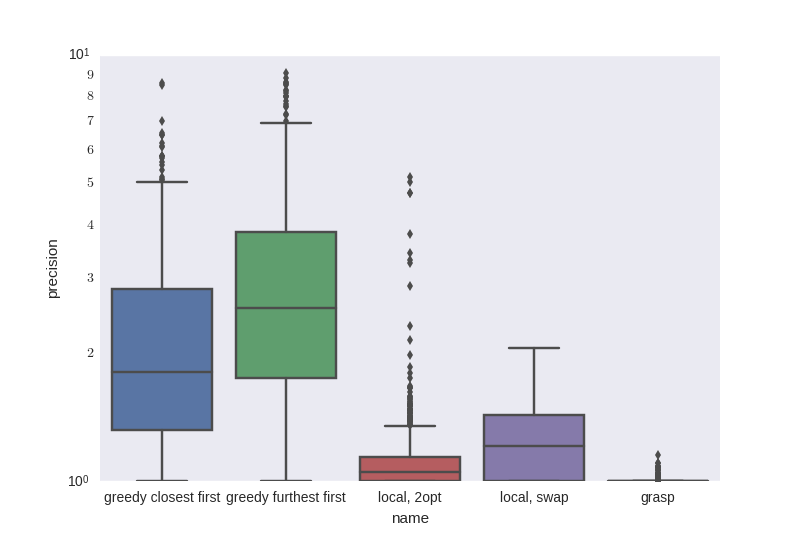
\includegraphics[width=12cm]{precision-big-all}
    \caption{Precisión comparando con el valor del mínimo en casos grandes}
    \label{fig:precision-big-all}
\end{figure}



\begin{table}[H]
    \begin{center}
        \begin{tabular}{ l | r }
            count  & 2008.000000 \\
            mean   &    1.111849 \\
            std    &    0.247017 \\
            min    &    1.000000 \\
            25\%   &    1.000000 \\
            50\%   &    1.049093 \\
            75\%   &    1.139941 \\
            max    &    5.181492 \\
        \end{tabular}
        \caption{Descripción de la precisión de la heurística local 2opt}\label{tab:precision-big-local-2opt}
    \end{center}
\end{table}

\subsubsection{Precisión en función del generador}

Utilizando las mismas variables descriptas en la sección \ref{sec:precision-big} generamos instancias con cada uno de los generadores disponibles, para ver si la precisión variaba con los tipos de problema.

El resultado puede verse en la figura \ref{fig:precision-big-all-bygen}.
Para las instancias de \texttt{zigzag} se suele conseguir buenos resultados en comparación con las \texttt{random}.
Ademas es notable que las instancias de \texttt{separated} se suelen resolver relativamente bien con las heurísticas locales y GRASP, no así con los greedy. Las conclusiones anteriores en comparaciones dentro de cada implementación parecen mantenerse.

\begin{figure}[H]
    \centering
    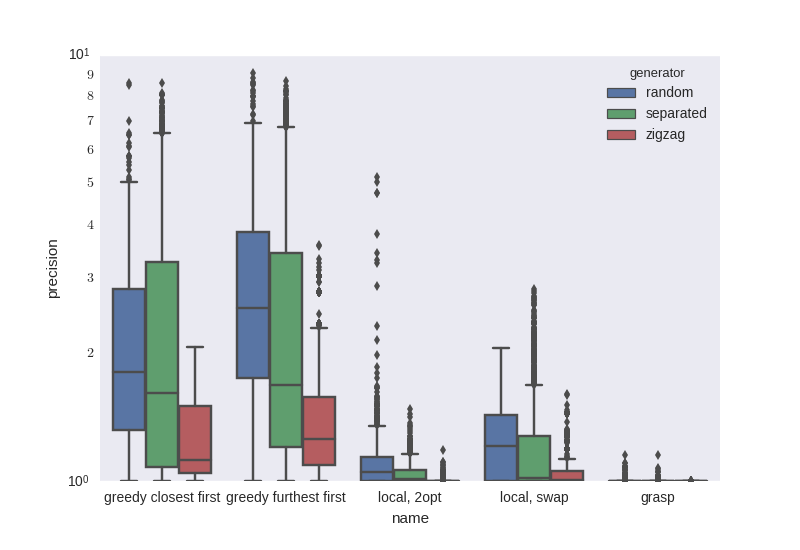
\includegraphics[width=12cm]{precision-big-all-bygen}
    \caption{Precisión comparando con el mínimo, según el generador utilizado}
    \label{fig:precision-big-all-bygen}
\end{figure}

\subsubsection{Precisión en función del tamaño de la mochila}

Quisimos también probar si el tamaño de las mochilas influía en la precisión de cada método.
Para ello tomamos los resultados obtenidos en la sección \ref{sec:precision-big} y los separamos
por el tamaño de la mochila relativo a la cantidad de paradas.

El resultado, que puede observarse en la figura \ref{fig:precision-big-all-bysize},
muestra una leve correlación para las heurísticas greedy. Las heurísticas locales y GRASP, en cambio, no parecen verse afectadas.

Tampoco se modifican las conclusiones entre implementaciones \emph{'Closest First vs Furthest First'}, \emph{'2opt vs Swap'} ó \emph{'GRASP Alternado vs GRASP 2opt'}.

\begin{figure}[H]
    \centering
    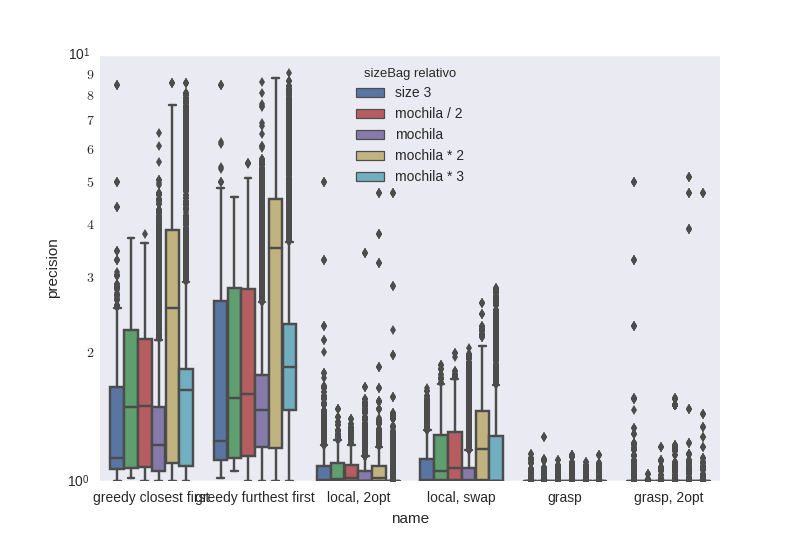
\includegraphics[width=12cm]{precision-big-all-bysize}
    \caption{Precisión comparando con el mínimo, según el tamaño relativo de la mochila}
    \label{fig:precision-big-all-bysize}
\end{figure}

\subsection{Variación de las variables del GRASP}

Cuando presentamos la metaheurística GRASP describimos dos variables que recibe como parámetro.
Por un lado la que llamaremos $inicios$, que se usa como exponente para calcular la cantidad de puntos de partida aleatorios a utilizar.
Y la otra, que llamaremos $limite$, que se usa como exponente para limitar la cantidad de pasos a dar por las búsquedas locales.

Para estudiar el comportamiento de la metaheurística al variar ambos exponentes generamos tres instancias del problema con 25 gimnasios,
25 paradas, y mochila de tamaño 100. Luego corrimos el GRASP variando cada exponente entre $0.2$ y $1.7$, en pasos de a $0.1$ y obtuvimos
los valores medios de tiempo y precisión (comparando con el mejor resultado) entre las tres instancias.

En la figura \ref{fig:grasp-variables-time} pueden apreciarse los tiempos obtenidos.
Se observa un claro comportamiento exponencial en función de la cantidad de $inicios$.
Por otro lado, encontramos que a partir de un $limite$ igual a 0.5 el tiempo deja de aumentar para este ya que
probablemente casi todas las búsquedas locales terminen en los pasos anteriores.

Al observar los cambios de precisión en la figura \ref{fig:grasp-variables-prec} vemos que nuevamente los resultados se mantienen constantes
al aumentar el $limite$ mas allá de 0.5. Vemos en cambio que los resultados van descendiendo siempre que aumentamos
la cantidad de inicios.

Comparando ambos gráficos se aprecia que los valores $1$ y $1$ utilizados como exponentes de $inicios$ y $limite$ en las mediciones
de la sección \ref{sec:time-grasp} brindan un buen tradeoff entre tiempo y precisión. Aunque si uno no buscara resultados tan exactos,
utilizar $0.4$ para ambos exponentes reduciría el tiempo de corrida en un $94\%$ a costa de obtener un resultado un $6\%$ peor.

\begin{figure}[H]
    \centering
    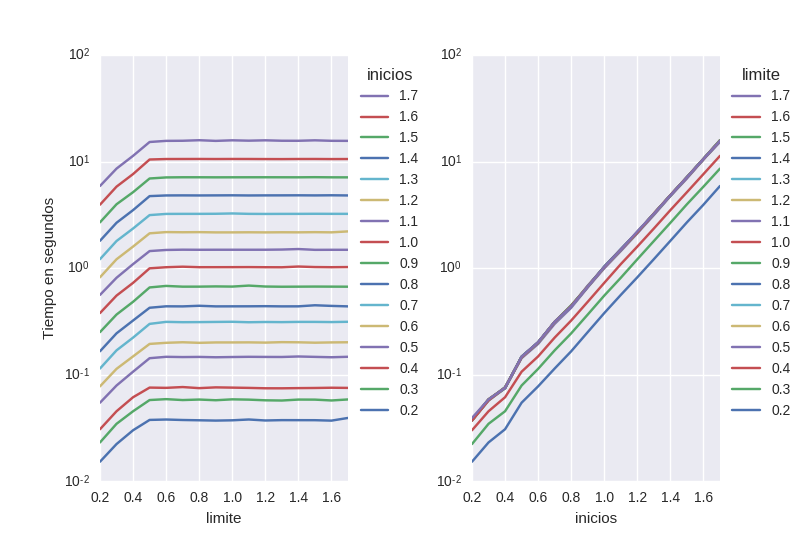
\includegraphics[width=14cm]{grasp-variables-time}
    \caption{Tiempo de corrida medio de GRASP al variar sus exponentes, sobre tres problemas con 50 nodos}
    \label{fig:grasp-variables-time}
\end{figure}

\begin{figure}[H]
    \centering
    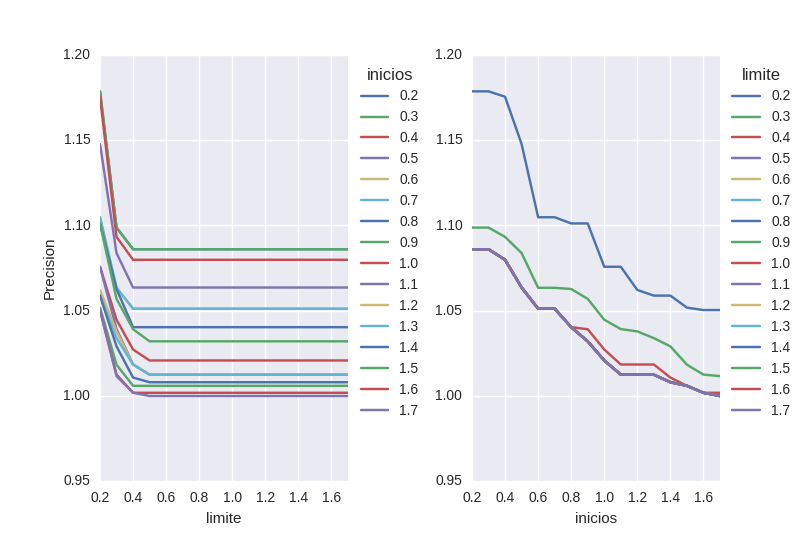
\includegraphics[width=14cm]{grasp-variables-prec}
    \caption{Precisión media de GRASP al variar sus exponentes, sobre tres problemas con 50 nodos}
    \label{fig:grasp-variables-prec}
\end{figure}

\subsection{Segundo set de muestras}

Para comprobar que las conclusiones obtenidas se correspondan con el verdadero comportamiento de los algoritmos
generamos un nuevo set de instancias aleatorias y corrimos nuevamente todas las mediciones.

A continuación presentamos los gráficos mas representativos de las secciones anteriores, correspondientes esta vez
al nuevo set de instancias.

\begin{figure}[H]
    \centering
    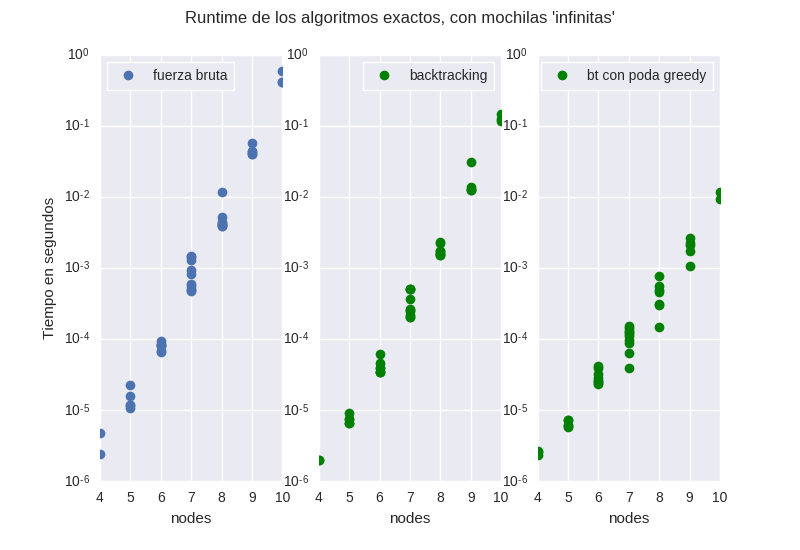
\includegraphics[width=12cm]{test-time-exacto}
    \caption{Tiempo de ejecución, en escala logarítmica, de los algoritmos exactos.}
    \label{fig:test-time-exacto}
\end{figure}

\begin{figure}[H]
    \centering
    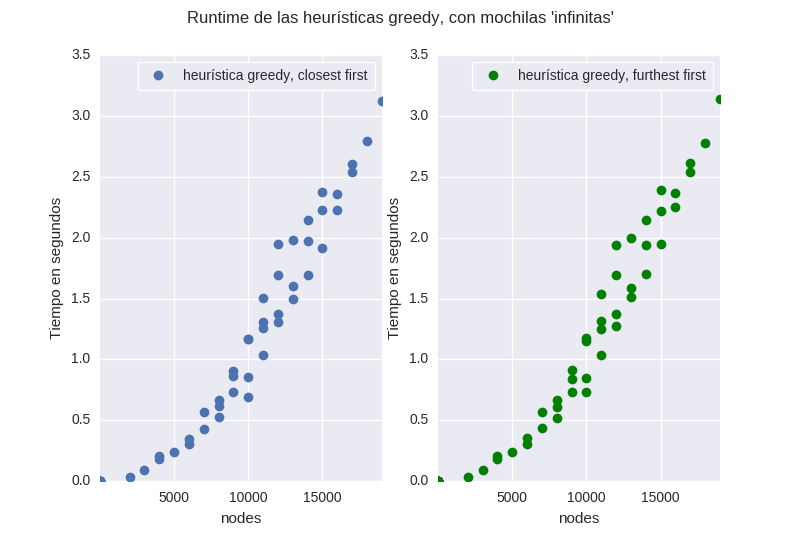
\includegraphics[width=12cm]{test-time-greedy}
    \caption{Tiempo de ejecución de las heurísticas greedy}
    \label{fig:test-time-greedy}
\end{figure}

\begin{figure}[H]
    \centering
    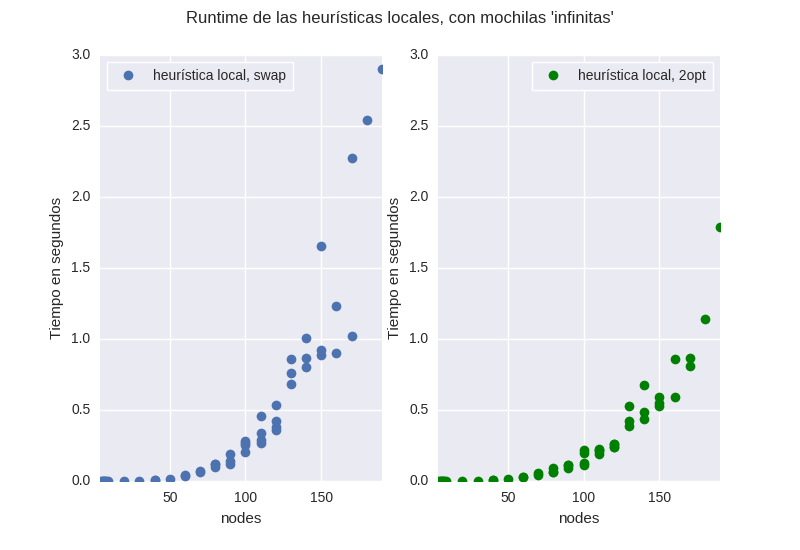
\includegraphics[width=12cm]{test-time-local}
    \caption{Tiempo de ejecución de las heurísticas locales}
    \label{fig:test-time-local}
\end{figure}

\begin{figure}[H]
    \centering
    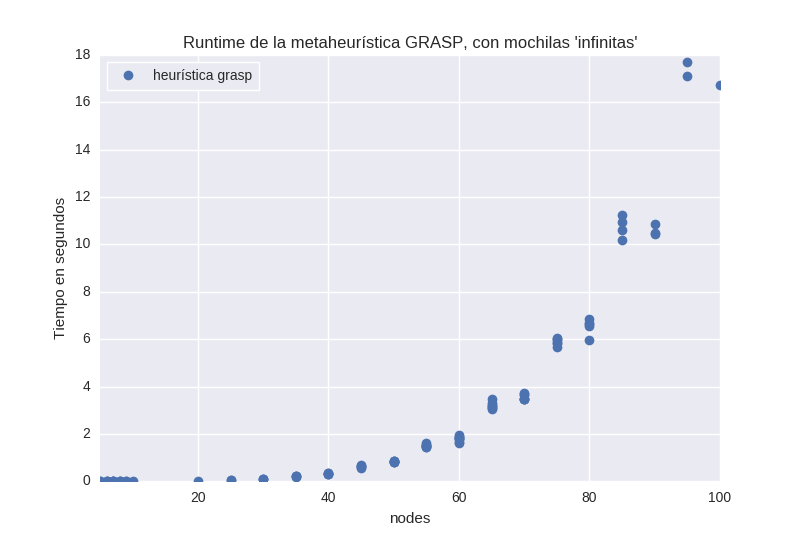
\includegraphics[width=12cm]{test-time-grasp}
    \caption{Tiempo de ejecución de la metaheurística grasp alternando búsquedas locales}
    \label{fig:test-time-grasp}
\end{figure}

\begin{figure}[H]
    \centering
    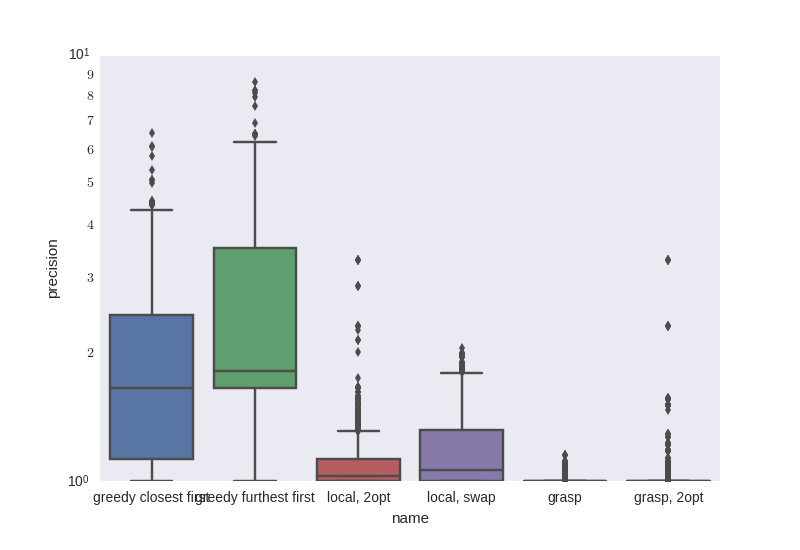
\includegraphics[width=12cm]{test-precision-big-all}
    \caption{Precisión comparando con el valor del mínimo en casos grandes}
    \label{fig:test-precision-big-all}
\end{figure}

\begin{figure}[H]
    \centering
    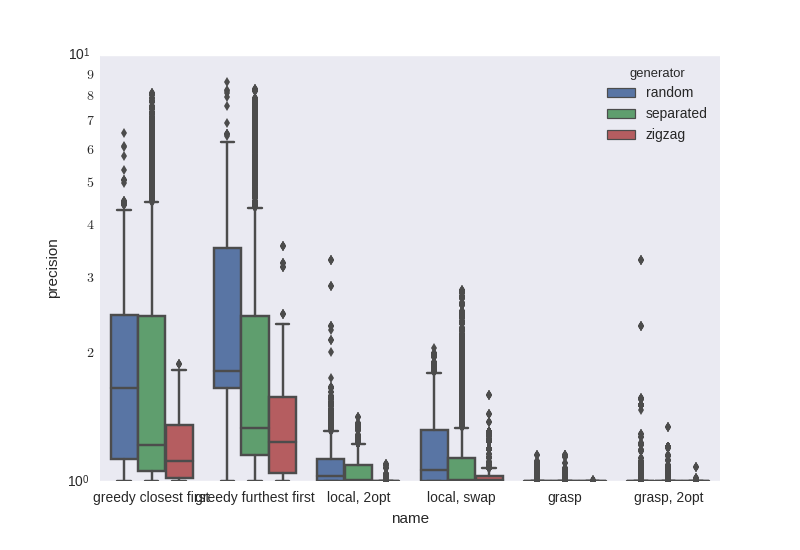
\includegraphics[width=12cm]{test-precision-big-all-bygen}
    \caption{Precisión comparando con el mínimo, según el generador utilizado}
    \label{fig:test-precision-big-all-bygen}
\end{figure}

Como podemos ver, en todos los casos los valores medidos presentan el mismo comportamiento que el analizado previamente.
